% https://tex.stackexchange.com/a/252261
\documentclass{beamer}
\usepackage{tikz}

\begin{document}

\begin{frame}
\begin{tikzpicture}

    \only<1->{
        \node[anchor=south west,inner sep=0] (A) at (0,0) {\includegraphics[width=.3\textwidth]{example-grid-100x100bp}};
    }

    \only<2->{
        \node[anchor=south west,inner sep=0] (B) at (4,0) {\includegraphics[width=.3\textwidth]{example-grid-100x100bp}};
        \fill [draw=none, fill=white, fill opacity=0.7] (A.north west) -- (A.north east) -- (A.south east) -- (A.south west) -- (A.north west) -- cycle;
    }

    \only<3->{
        \node[anchor=south west,inner sep=0] (C) at (8,0) {\includegraphics[width=.3\textwidth]{example-grid-100x100bp}};
        \fill [draw=none, fill=white, fill opacity=0.7] (B.north west) -- (B.north east) -- (B.south east) -- (B.south west) -- (B.north west) -- cycle;
    }

\end{tikzpicture}
\end{frame} 

\end{document}
